\begin{frame}[shrink=30]{Learning Stages}
	\begin{center}
		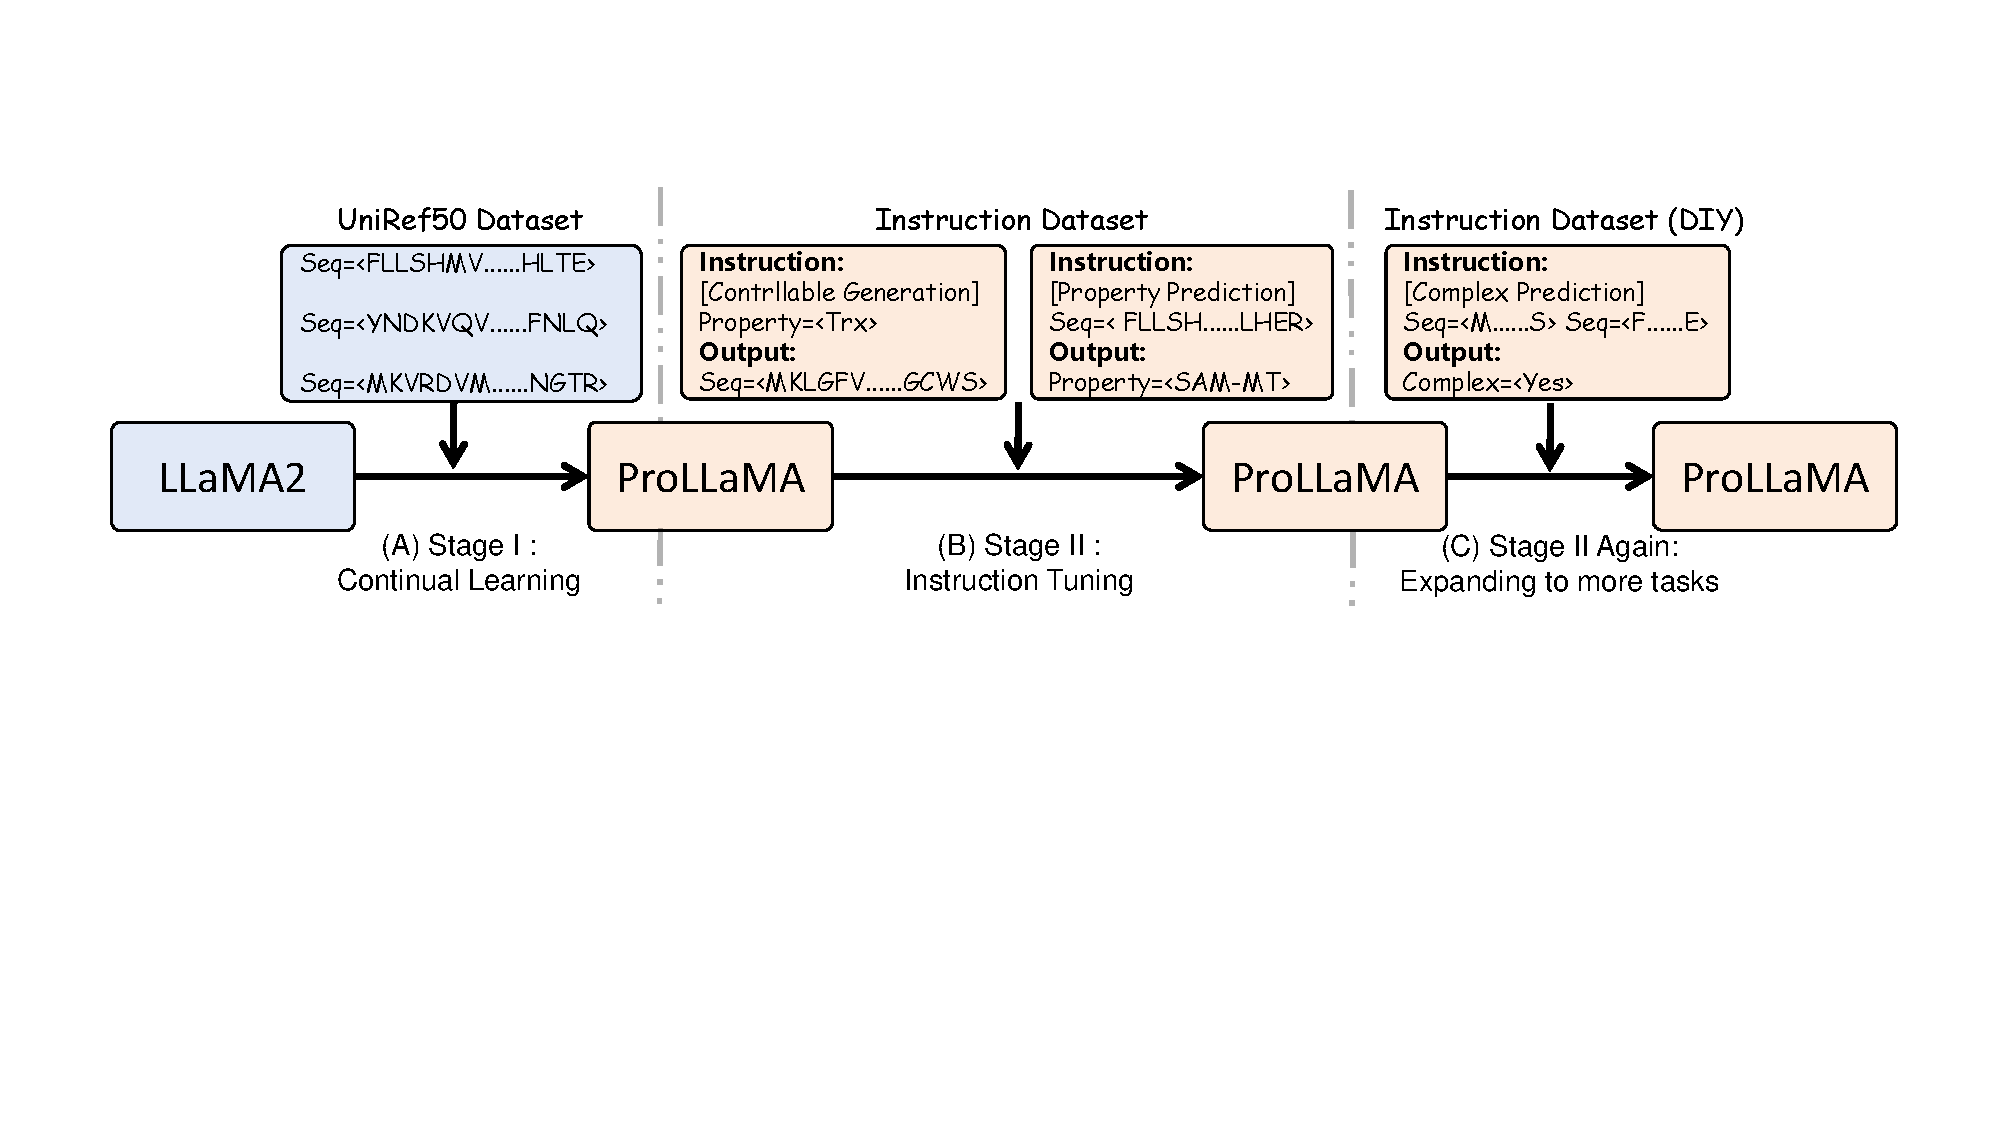
\includegraphics[scale=0.5]{images/training.pdf}
	\end{center}
	\credit{Image}{lv2024prollama}
	\begin{itemize}
		\item Stage I
		\begin{itemize}
			\item reuses pre-trained general LLM for NLP (e.g., LLaMA2)
			\item learns protein language
			\item trains decoder's LoRA
			\item includes both the Embed and Generation Head layers in training
			\begin{itemize}
				\item a token may have different meanings in protein
				sequences and natural languages, requiring distinct embeddings for the same token.
			\end{itemize}
		\end{itemize}
		\item Stage II
		\begin{itemize}
			\item learns to follow instructions
			\item multiple tasks
			\item trains only decoder's LoRA at a lower rank than Stage I
		\end{itemize}
		\item More stages
		\begin{itemize}
			\item more tasks
			\item optional
		\end{itemize}
		\item preserves natural language abilities
	\end{itemize}
\end{frame}